\documentclass[11pt]{article}
\usepackage{multicol}
\setlength{\columnseprule}{1pt} % separation line between columns
\setlength{\parindent}{0pt} % paragraph indentation

\usepackage[top=2cm, bottom=2cm, left=2cm, right=2cm]{geometry}
\usepackage[T1]{fontenc}
\usepackage[utf8]{inputenc}
\usepackage[francais]{babel}
\usepackage{textcomp}

\usepackage{hyperref}
\hypersetup{
	colorlinks=true,       	% false: boxed links; true: colored links
	linkcolor=black,          	% color of internal links
	urlcolor=blue,           	% color of external links
	citecolor=blue
}

\usepackage{dashrule}
\usepackage{wrapfig}
\usepackage{graphicx}
\usepackage{enumitem}
\usepackage{wrapfig}
\usepackage{cancel} % diagonal strikeout
\usepackage[margin=1cm]{caption}
\usepackage{subcaption}
\setdescription{leftmargin=1cm,labelindent=0.5cm}

\usepackage{amsmath}
\usepackage{amssymb}
\usepackage{amsfonts}

\newcommand\mathd[0]{\mathrm{d}} 

\usepackage{blindtext}

% Colors
\usepackage[usenames,dvipsnames]{xcolor}
\definecolor{session_bg}{RGB}{25,25,25}
\definecolor{grey}{rgb}{0.96,0.96,0.96}
\definecolor{grey2}{rgb}{0.3,0.3,0.3}
\definecolor{dkgreen}{rgb}{0,0.6,0}
\definecolor{gray}{rgb}{0.5,0.5,0.5}
\definecolor{mauve}{rgb}{0.58,0,0.82}
\definecolor{blue}{rgb}{0,0,0.7}

% Colored frame
\usepackage{framed}
\definecolor{shadecolor}{rgb}{0.96,0.96,0.96}
\definecolor{TFFrameColor}{rgb}{0.96,0.96,0.96}
\definecolor{TFTitleColor}{rgb}{0.00,0.00,0.00}

% Redefine leftbar environment
\newlength{\leftbarwidth}
\setlength{\leftbarwidth}{1pt}
\newlength{\leftbarsep}
\setlength{\leftbarsep}{10pt}

\newcommand*{\leftbarcolorcmd}{\color{leftbarcolor}} % as a command to be more flexible
\colorlet{leftbarcolor}{gray}

\renewenvironment{leftbar}{%
    \def\FrameCommand{{\leftbarcolorcmd{\vrule width \leftbarwidth\relax\hspace {\leftbarsep}}}}%
    \MakeFramed {\advance \hsize -\width \FrameRestore }%
}{%
    \endMakeFramed
}

\usepackage{listings}
\lstset{
	numbers=left,                   % where to put the line-numbers
    language=C++,
	tabsize=4,
	frame=single,                   % adds a frame around the code
	breaklines=true,				% text wrapping
    basicstyle=\scriptsize\ttfamily,
    numberstyle=\scriptsize\ttfamily,
    backgroundcolor=\color{grey},
    showstringspaces=false,
    keywordstyle=\color{OliveGreen},
    stringstyle=\color{BrickRed},
    commentstyle=\color{grey2}\it,
	emphstyle=\color{mauve},
    stepnumber=1
}


% Title page
\title{Création d'une interface graphique et interactive \\ pour jeux de rôles papier}
\author{
	Damien Martel \\ \href{mailto:damien.martel@edue.esiee.fr}{damien.martel@edu.esiee.fr} \and
	Bertrand Le Mée \\ \href{mailto:bertrand.lemee@edu.esiee.fr}{bertrand.lemee@edu.esiee.fr} \and
	Vincent Lindivat \\ \href{mailto:vincent.lindivat@edu.esiee.fr}{vincent.lindivat@edu.esiee.fr} \and
	Frédéric Nguyen \\ \href{mailto:frederic.nguyen@edu.esiee.fr}{frederic.nguyen@edu.esiee.fr}
}
\date{\today}

\begin{document}
\maketitle
\newpage
\hfill
\newpage
\tableofcontents
\newpage

\section{Introduction}

Le jeu de rôle (JdR) papier permet à un groupe de joueurs, réunis dans la même salle, d'incarner des personnages dans un univers fictif. Un Maître du jeu (MJ) les guide dans cet univers, leur proposant problèmes, quêtes et discussions avec d'autres personnages fictifs, et orchestrant l'ensemble de la partie, ou "session". Afin de rendre l'univers plus immersif, de nombreux supports physiques sont utilisés: cartes, dés, plateaux, jetons, dessins...\\
Cependant, il n'est pas toujours possible de réunir l'ensemble du groupe pour une session, selon les emplois du temps personnels. Cela mène à des entorses scénaristiques, notamment lors de l’absence d'un personnage possédant des informations clés pour l'aventure.\\

Ayant ces éléments à l'esprit, nous avons développé une interface graphique qui permet d'organiser des parties de jeu de rôle à distance sur réseau. Nous avons fait attention à ne pas dépayser les utilisateurs en conservant au mieux l'atmosphère du jeu de plateau habituel.\\

Ce projet est une opportunité pour nous de découvrir le travail de développement en équipe sur un projet de plus grande envergure que ce que nous avons réalisé jusqu'à maintenant.	
\newpage

\section{Méthode agile SCRUM}

A l'occasion de ce projet, nous avons pu découvrir la méthode de développement
 agile SCRUM  et dans le même mouvement, appliquer cette méthode à la réalisation de notre projet.\\
 
Dans le cadre SCRUM, les trois entités suivantes se rassemblent autour du projet :

\begin{description}
	\item[Product Owner] \hfill \\
		Il définit les fonctionnalités du projet et décide de valider ou non les résultats. Il met en place les dates à respecter. Le Product Owner établit aussi le \textit{Backlog} avec le Scrum Master et l'équipe, mais il peut modifier un \textit{Sprint} si besoin.
	\item[Scrum Master] \hfill \\
		Il s'occupe de l'équipe de développement en veillant à ce la méthode SCRUM soit bien appliquée. Il conseille son équipe et s'assure qu'elle progresse correctement. Il gère aussi les relations extérieures, particulièrement avec le Product Owner.
	\item[Equipe de développement] \hfill \\
		Généralement constituée de 5 à 10 personnes, l'équipe regroupe tout type de rôle. Une équipe travaille sur un \textit{Sprint} et est libre de s'organiser d'elle-même.
\end{description}

La progression du projet est basée sur un \textbf{Backlog}, faite par le Product Owner, le Scrum Master et l'équipe, qui est une liste ordonnée par priorité et complexité de temps de tâches à réaliser. Les priorités sont choisies par le Product Owner et peuvent être revues selon le courant des événements. \\

Durant le projet, le temps est divisé en séquence ayant une durée moyenne de 2 semaines, ces séquences sont appelées \textbf{Sprint}. Avant chaque Sprint, l'équipe choisit dans le Backlog l'ensemble des tâches qu'elle compte pouvoir réaliser. \\

Quotidiennement, une réunion d'une quinzaine de minutes \textbf{debout} se fait dans l'équipe afin de faire le point sur ce qui a été fait le jour précédent et ce qui va être fait le jour de la réunion. Lorsqu'un Sprint est terminé, le Product Owner, le Scrum Master et l'équipe se rassemble pendant 30 minutes pour faire le point ce qui a marché et ce qui n'a pas marché afin de mieux préparer et agir lors du prochain Sprint. \\

N'étant qu'une équipe de 4 et le projet ne durant que 2 mois, nous avons dû réadapter la méthode. Nous nous sommes convenus de faire des Sprints de une semaine et travailler de façon très souple pendant les temps de travail.
\newpage

\section{Évolution de l'interface graphique}

Étant donné que nous appliquons la méthode SCRUM, le projet subit de nombreuses modifications au fur et à mesure que le projet avance. Procédant par itération, nous découvrons des contraintes avec l'interface que nous utilisons comme opportunités pour apporter des améliorations pour accueillir les fonctionnalités à ajouter. 

\begin{figure}[h!]
	\centering
	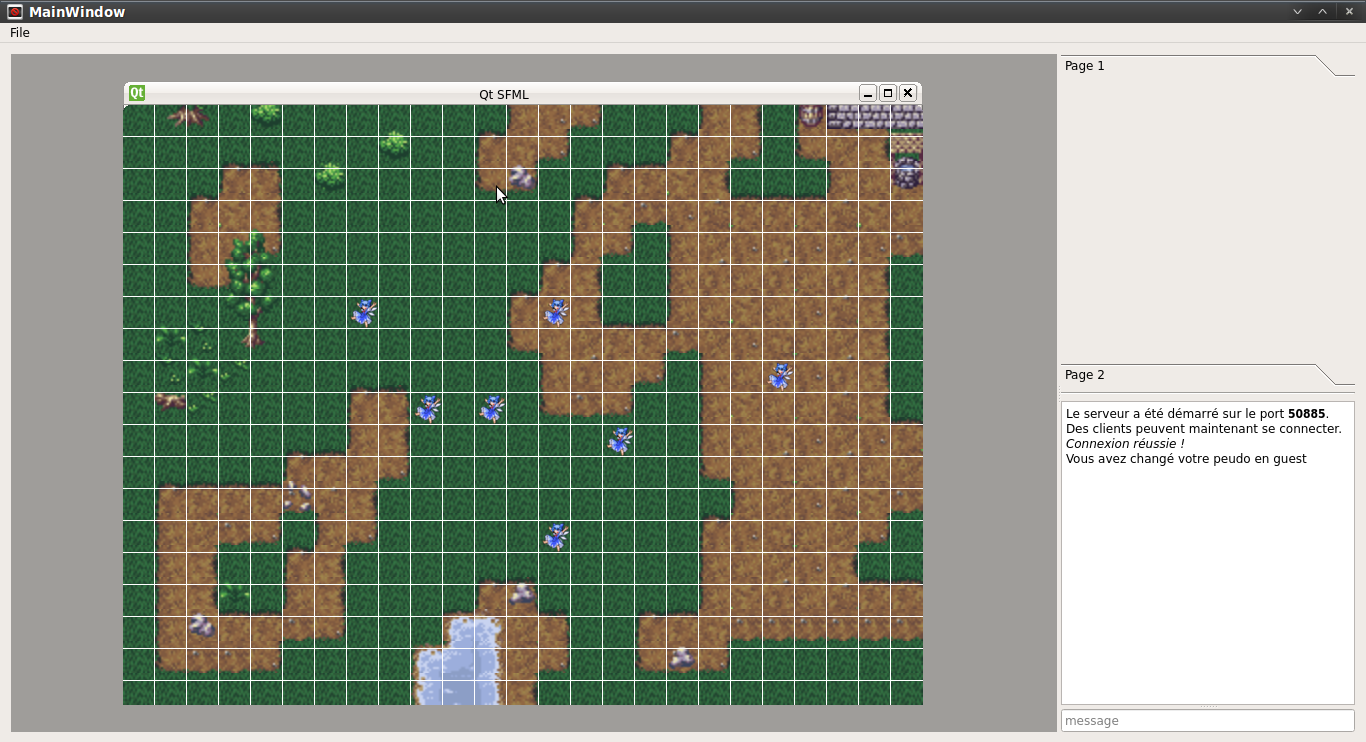
\includegraphics[width=0.8\textwidth]{img/gui_history/2014_05_07_screen.png}
	\caption{Interface du 7 Mai 2014}
\end{figure}

\begin{figure}[h!]
	\centering
	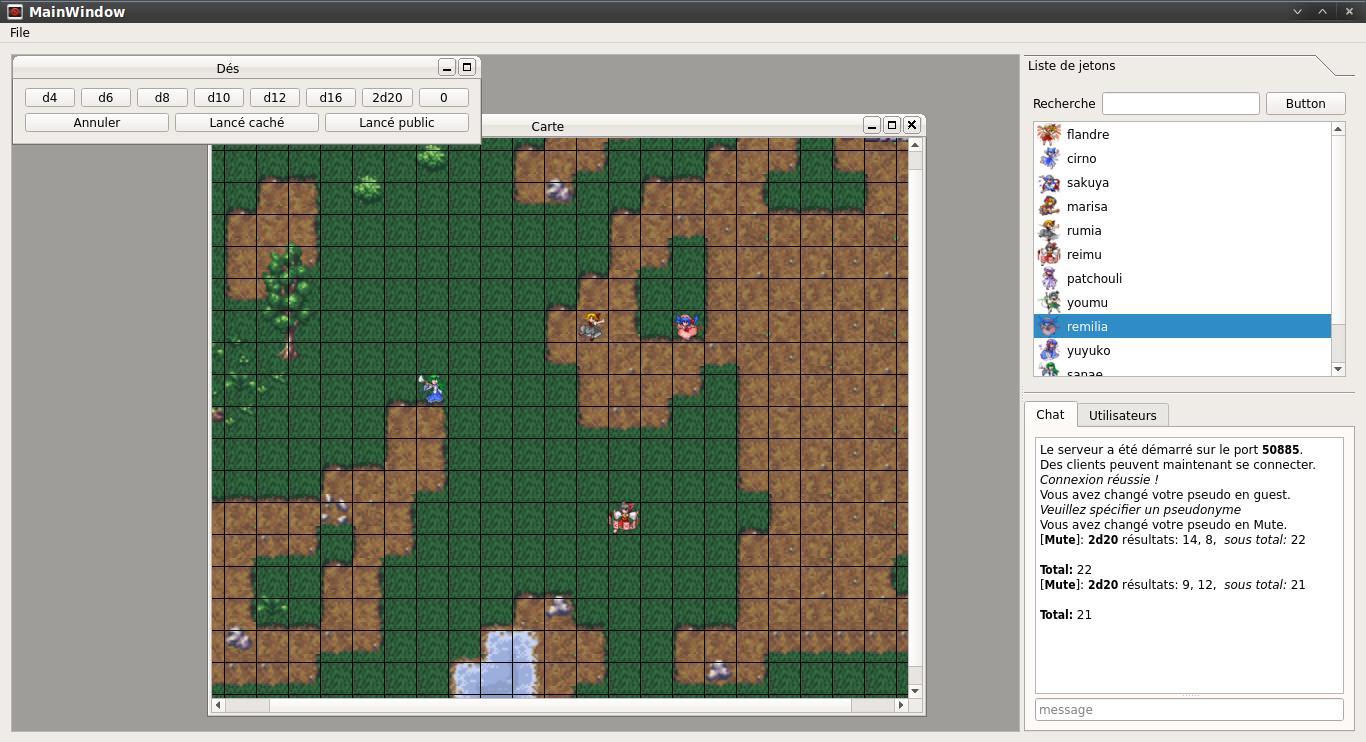
\includegraphics[width=0.8\textwidth]{img/gui_history/2014_05_21_screen.png}
	\caption{Interface du 21 Mai 2014 - Ajout des dés}
\end{figure}
\newpage

\begin{figure}[h!]
	\centering
	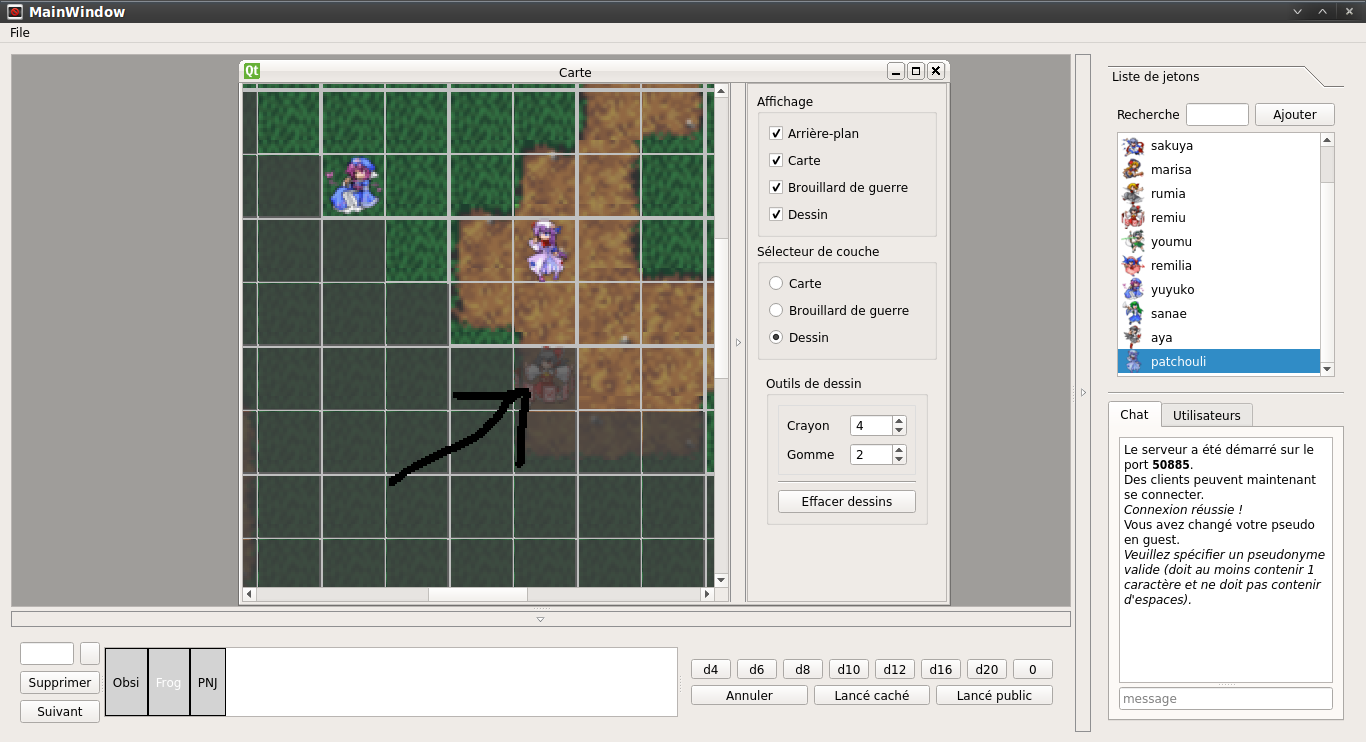
\includegraphics[width=0.8\textwidth]{img/gui_history/2014_05_30_screen.png}
	\caption{Interface du 30 Mai 2014 - Ajout du gestionnaire de tour + outils de carte}
\end{figure}

\begin{figure}[h!]
	\centering
	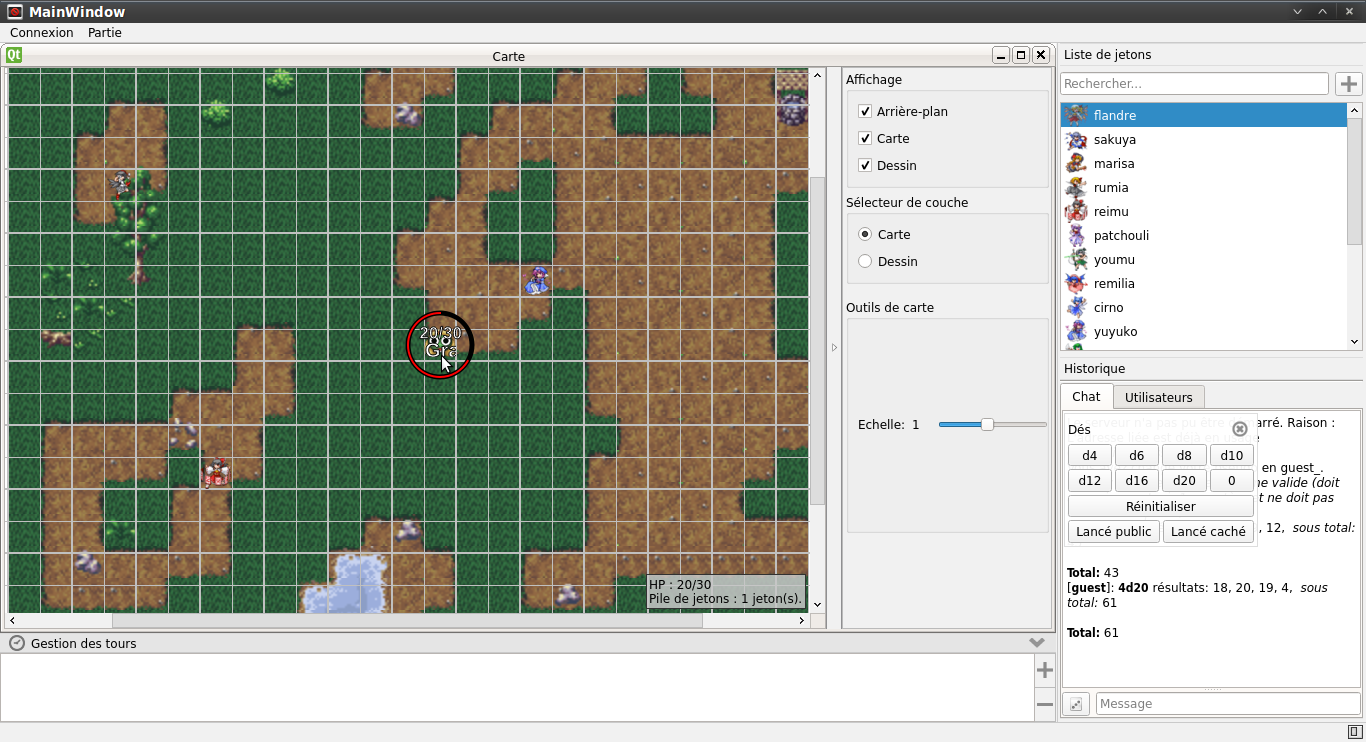
\includegraphics[width=0.8\textwidth]{img/gui_history/2014_06_18_screen.png}
	\caption{Interface du 18 Juin 2014 - Changement du style graphique}
\end{figure}

\newpage

\section{Manuel d'utilisation}

Cette application débute avec une boîte de dialogue qui laisse le choix entre deux rôles : Maître de Jeu (MJ) ou Joueur. Si "MJ" est choisi, l'application se met en tant que serveur pour accueillir les joueurs. Si "Joueur" est choisi, un assistant ce connexion apparaît pour choisir à quel serveur se connecter. \\

L'interface qui se présente comporte un Chat, un gestionnaire de tours et le lanceur de dés. Le Chat contient la liste des utilisateurs et permet aux joueurs et au MJ de communiquer. De plus, le chat possède des commandes qui s'introduisent par un /. Les commandes implémentées sont :

\begin{description}
	\item[/help] \hfill \\
		Affiche l'ensemble des autres commandes disponibles du chat avec les indications d'utilisation.
	\item[/nickname <pseudo>] \hfill \\
		Modifie le pseudo par celui qui suit la commande.
	\item[/roll <nombre de dés>d<valeur max du dé>] \hfill \\
		Roule un nombre de fois voulu du dé choisi. Peut s'utiliser en chuchotement.
	\item[/whisper <utilisateur> <message>] \hfill \\
		Envoie un message privé au joueur indiqué.
\end{description}

\begin{figure}[h!]
	\centering
	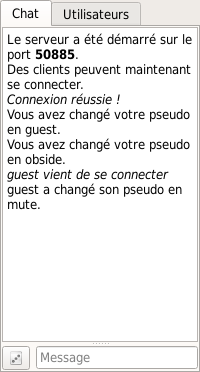
\includegraphics[scale=0.5]{img/chat_mj.png}
	\hspace{10 mm}
	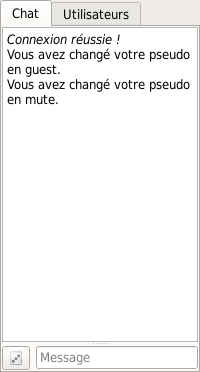
\includegraphics[scale=0.5]{img/chat_player.png}
	\caption{Chat MJ (à gauche) et chat Joueur (à droite)}
\end{figure}

Le Chat propose également une liste d'utilisateurs connectés. Un clic droit sur un ou plusieurs utilisateurs de cette liste affiche un menu contextuel donnant accès à des actions : Envoyer un message, et Lancer les dés.
La première action prépare un message privé à un ou plusieurs utilisateurs, la seconde lance les dés sélectionnés dans le lanceur de dés et envoie le résultat aux utilisateurs sélectionnés.


\begin{figure}[h!]
	\centering
	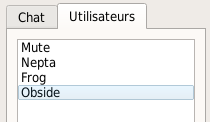
\includegraphics[scale=0.5]{img/chat_userlist_1.png}
	\hspace{10 mm}
	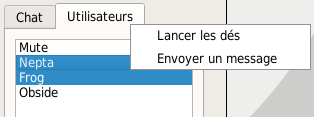
\includegraphics[scale=0.5]{img/chat_userlist_2.png}
	\caption{Liste d'utilisateurs (à gauche) et menu contextuel proposant des actions sur les utilisateurs sélectionnés (à droite)}
\end{figure}

Le lanceur de dés propose les dés les plus utilisés et permet de choisir pour chaque type de dé, le nombre de fois que celui-ci doit être lancé. Initialement, les compteurs sont à zéro. Pour augmenter le nombre de fois que l'on lance un dé, il faut appuyer sur le bouton correspondant ou utiliser la molette de la souris pour faire varier le nombre en étant sur le bouton. On peut ensuite décider de lancer les dés sur le chat (lancé public) ou de lancer les dés en privé si le MJ l'exige (lancé caché). Il est possible de réinitialiser tous les compteurs.

\begin{figure}[h!]
	\centering
	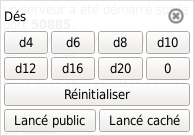
\includegraphics[scale=0.5]{img/dice_manager.png}
	\caption{Lanceur de dés}
\end{figure}

Le gestionnaire de tours est un outil qui permet au MJ de gérer ses combats. Il peut ajouter les joueurs ou personnages non joueurs (PNJ) en écrivant dans le champ de texte prévu à cet effet. Lorsque des utilisateurs se connectent, ils sont automatiquement ajoutés dans le gestionnaire de tour. Le MJ peut réordonner les tours à sa guise et dispose d'un certain nombre d'outils. Il peut ajouter des personnages comme dit précédemment, retirer un personnage à l'aide d'un bouton, déplacer les personnages dans le gestionnaire à la souris. Il dispose également de raccourcis clavier, par exemple les flèches du clavier permettent de naviguer entre les tours et de les réarranger.

\begin{figure}[h!]
	\centering
	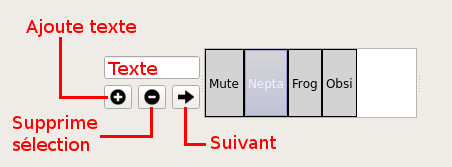
\includegraphics[scale=0.7]{img/turn_manager.jpg}
	\caption{Gestionnaire de tour}
\end{figure}
\newpage

\section{Aspects techniques}

\section{SFML}

Au début de notre projet, nous avions pensé à utiliser une bibliothèque graphique spécialisée dans la réalisation de jeu, SFML (\textit{Simple and Fast Multimedia Library}).\\

Cette bibliothèque nous aurait permis de réaliser facilement des animations et toute sorte d'effet graphique. 
Cependant, en utilisant SFML, de mauvaises réactions ont été constatées, notamment au niveau de l'affichage de la fenetre SFML.
Après plusieurs difficultés à faire cohabiter Qt et SFML, nous avons, au bout de deux semaines, nous avons décidé de réaliser l'application exclusivement avec Qt. Pour cela, nous avons dû repenser entièrement le système de carte déjà réalisé avec SFML.
\newpage

\subsection{Réseau}

% TODO insérer schéma UML

Lorsque l'application ne possédait qu'un chat, toutes les opérations nécessitant une mise en réseau se faisaient dans les classes gérant le Chat. Nous avons par la suite fait une refonte pour gérer plusieurs modules réseau en évitant de la duplication de code.\\

Nous avons tout d'abord pensé la mise en réseau sans nous occuper de la base de données. Nous avons donc cherché à pouvoir envoyer n'importe quel type d'objet. Pour cela, nous avons créé une interface Serializable possédant deux méthodes abstraites, \emph{serialize} et \emph{unserialize}. Toute classe pour laquelle nous souhaitons envoyer des objets sur le réseau doit implémenter l'interface Serializable et redéfinir les deux méthodes citées précédemment. La méthode \emph{serialize} doit stocker les attributs nécessaires à la reconstruction d'un objet de la classe dans un QByteArray. La méthode unserialize doit faire l'opération inverse, c'est à dire reconstruire un objet à partir d'un QByteArray.\\
Au final, nous n'avons que la classe Message implémentant l'interface Serializable, notre vision de la mise en réseau ayant changée pendant l'ajout de la base de donnée à l'application. En effet, notre première vision était d'envoyer des objets de classes implémentant l'interface Serializable à travers le réseau, nous aurions par exemple envoyé des objets de la classe Sprite. Cependant, avec la base de données nous avons plutôt pris l'approche suivante: les objets sont stockés en base de données, puis une notification est envoyé à toutes les applications afin que celles-ci récupèrent les nouvelles données présentes dans la base de données distante.\\

Pour communiquer, nous devons utiliser des sockets. Nous utilisons les classes présentes dans Qt: QTcpServer et QTcpSocket. Une QTcpSocket peut se connecter à un QTcpServer, et le QTcpServer reçoit un signal exploitable lorsqu'un client se connecte à lui. A travers ces sockets, des paquets sont envoyés. Nos paquet sont organisés de la manière suivante :\\

\begin{figure}[h!]
	\centering
	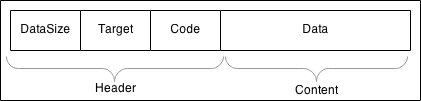
\includegraphics[scale=0.6]{img/network_packet.png}
	\caption{Structure d'un paquet}
\end{figure}

Un Header contient tout d'abord la taille de la donnée qui va être reçue, ce qui est nécessaire pour savoir lors de la réception si le paquet reçu est complet ou s'il faut attendre d'avoir reçu de nouvelles données. La Target correspond à un entier identifiant le module qui doit recevoir le paquet. Le Code correspond à l'action qui doit être effectuée par le module à qui le paquet à été transféré.\\

Lorsqu'un message est reçu, celui-ci passe par une classe héritant de Switch: SwitchClient ou SwitchServer. Ces classes sont les premières à recevoir le message et décident du module sur lequel le message doit être envoyé à l'aide de la target dans le header du paquet.\\

Les modules qui reçoivent des paquets héritent de Sender et Receiver. Un Receiver reçoit une donnée d'un Switch et la traite en exécutant des actions (méthode \emph{processNewData}). Un sender peut envoyer un paquet à une ou plusieurs sockets: un SenderClient pourra envoyer un paquet à la socket du serveur, et un SenderServer pourra envoyer un paquet à une ou plusieurs Socket(s) qui sont connectées à la socket serveur.\\

\subsubsection{MapClient \& MapServer}
Les cartes font partie des éléments mis en réseau dans l'application. La classe MapClient regarde le code du paquet reçu et exécute une action spécifique en fonction du code reçu. La classe MapServer quant à elle se contente de redistribuer les paquets qu'elle reçoit à toutes les applications (sauf l'émetteur du paquet reçu par MapServer).\\

Les actions disponibles sont les suivantes :
\begin{description}
	\item[Ouverture d'une carte] Le message reçu pour cette action contient l'id de la carte à ouvrir. Cette carte est récupérée de la base de données grâce à son id et est envoyée à la fenêtre principale pour que les initialisations nécessaires soit effectuées.
	\item[Ajout d'un sprite] L'action d'ajout d'un sprite récupère tout d'abord le sprite à ajouter de la base de données grâce à son id, récupère le jeton associé parmi les jetons déjà chargés dans l'applications et récupère la couche sur laquelle le sprite doit être posé avant de l'y ajouter.
	\item[Suppression d'un sprite] Le message de cette action contient l'id du sprite à supprimer et l'id de la couche sur laquelle celui-ci se situe. Cette couche est tout d'abord récupérée parmi les couches déjà chargées par l'application, puis nous récupérons le jeton posé sur cette couche grâce à son id. Une fois le pointeur vers ce jeton récupéré, celui-ci est supprimé.
	\item[Suppression de tous le FoW] Cette action fonctionne sur le même principe que la suppression d'un sprite, la couche de brouillard de guerre est tout d'abord récupérée grâce à son id, puis tous les sprites de cette couche sont supprimés.
	\item[Mise à jour de la couche de dessin] La couche de dessin ayant été mise à jour est tout d'abord récupérée de la base de données, puis la pixmap (image) en est extraite. Cette pixmap est remplacée dans la couche de dessin concernée.
	\item[Ping] Un message contenant l'id de la couche sur laquelle afficher le ping, ainsi que sa position en x et en y est reçu. L'action récupère ces informations, et fait appel à l'outil de ping de la couche de dessin concernée en lui passant la position en paramètre.
\end{description}
\bigskip

Ces actions sont de simples méthodes dans la classe MapClient, une évolution possible aurait été de créer une classe Action, avec plusieurs classes héritant de celle-ci pour les différentes actions de MapClient. Ces actions auraient été créées lors d'un événement sur la carte (par exemple un clic de souris pour ajouter un jeton), puis envoyées via le réseau, puis exécutées sur les différents clients lors de la réception. Cela aurait eu plusieurs bénéfices : 
\begin{itemize}
	\item ces actions auraient été génériques, afin d'être réutilisées pour tous les modules réseau de l'application;
	\item ces actions auraient pu être réversibles (une liste au niveau de MapServer garderait une trace des actions effectuées);
	\item logger les actions aurait été plus simple qu'à l'heure actuelle.
\end{itemize}
\bigskip

De plus, l'ordre dans lequel les étapes sont effectuées pour ces actions est difficilement exploitable, notamment pour des fonctionnalités de modérations. Prenons l'exemple de l'ajout d'un Sprite sur une carte décrit sur la figure \ref{fig:network_addsprite}.
\newpage

\begin{figure}[h!]
	\centering
	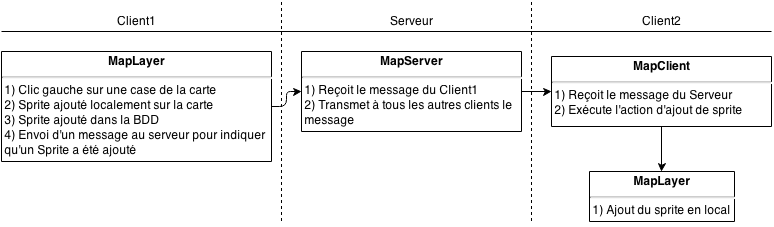
\includegraphics[width=1.0\textwidth]{img/network_addsprite.png}
	\caption{Etapes pour l'ajout d'un Sprite}
	\label{fig:network_addsprite}
\end{figure}

Dans le cas actuel décrit ci-dessus, sur un clic gauche de la souris sur la carte, un sprite est ajouté sur la carte localement et en base de données. Cependant, si nous voulons effectuer de la modération du côté du serveur, cela complique la tâche : en effet le sprite a déjà été ajouté à un client et en base de données. Il faudrait que les étapes s'effectuent comme sur le schéma ci-dessous :

\begin{figure}[h!]
	\centering
	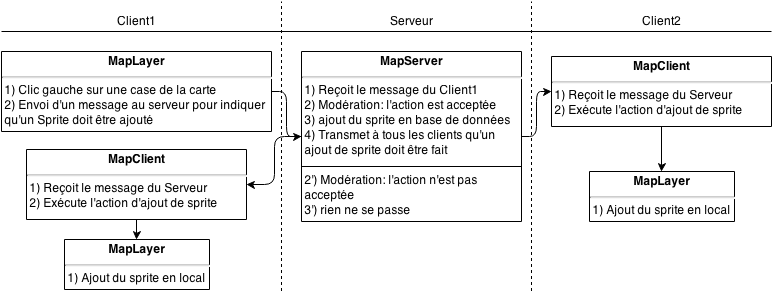
\includegraphics[width=1.0\textwidth]{img/network_addsprite_better.png}
	\caption{Etapes pour l'ajout d'un Sprite (amélioré)}
\end{figure}

\textbf{N.B.} TokenMenuClient, TokenMenuServer, TurnMenuClient et TurnMenuServer reprennent le même principe que MapClient et MapServer et ne sont donc pas détaillés.

\subsubsection{ChatClient \& ChatServer}
Les classes ChatClient et ChatServer récupèrent le code présent dans le header d'un paquet reçu et récupèrent la commande associée. Une commande est représentée par un objet d'une classe héritant de AbstractCmd. Le principe du Chat ainsi que les différentes commandes sont détaillés dans la sous-section concernant le Chat dans la section aspects techniques. Nous pouvons cependant noter que ChatClient et ChatServer utilisent des commandes, tandis que MapClient, MapServer et les autres modules utilisent des actions sous forme de méthode. Comme détaillé précédémment, il aurait été judicieux de créer des classes héritant d'une classe de base Action qui soit générique afin d'être réutilisable dans toute l'application, contrairement aux commandes qui sont fortement liées au chat.
\newpage

\subsection{Chat}

\begin{figure}[h!]
	\centering
	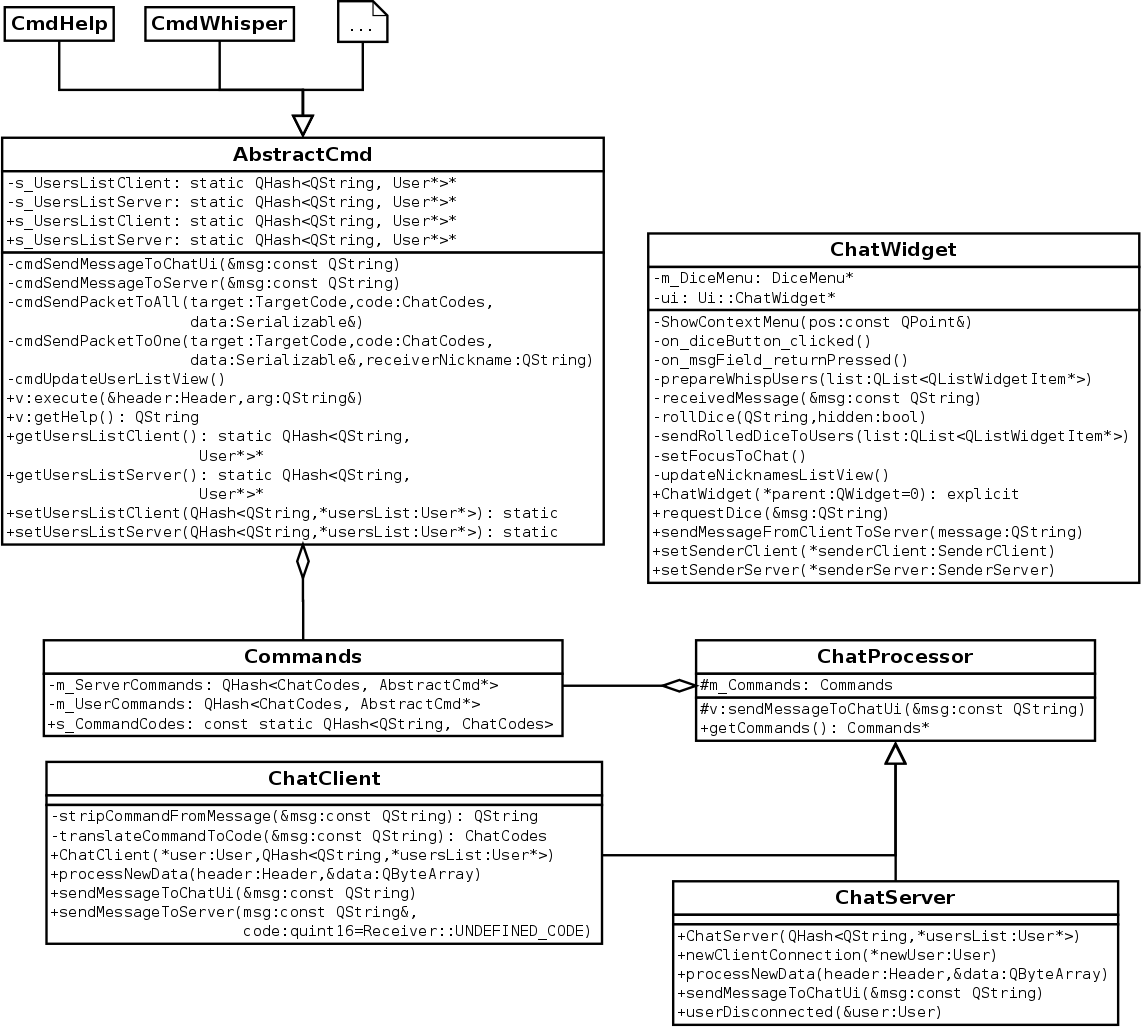
\includegraphics[width=\textwidth]{img/chat_uml.png}
	\caption{Diagramme UML du chat (seules quelques commandes ont été représentées pour éviter de surcharger le schéma)}
\end{figure}

Au début du projet, la base du chat s'est construite à l'aide de la partie \emph{Communiquer en réseau avec son programme} provenant du tutorial \emph{Programmez avec le langage C++} de OpenClassrooms \cite{cite:oc:cpp}, tutorial que nous avons également utilisé avant le début du projet pour revoir les bases du C++ et avoir une brève introduction à Qt.\\

Le Chat est constitué de la classe ChatWidget qui fait le lien entre l'interface graphique et les commandes qui peuvent être exécutées.\\

Lorsqu'une application est lancée, le pseudo souhaité par l'utilisateur est tout d'abord demandé. Ce pseudo n'est pas tout de suite utilisé, il est sauvegardé dans un attribut, et l'utilisateur est temporairement nommé \emph{guest}. La QTcpSocket se connecte ensuite au QTcpServer du MJ, et la méthode newClientConnection de ChatServer est appelée du côté du MJ. Cette méthode vérifie si le pseudo \emph{guest} est déjà pris et ajoute un tiret bas à la fin si c'est le cas (\emph{guest\_}), puis crée un User et l'ajoute à la liste des utilisateurs de SwitchServer et des modules réseau (ChatServer, MapServer, ...). Un message est ensuite envoyé au ChatClient de l'utilisateur venant de se connecter afin de le notifier de sa connexion et de son éventuel changement de pseudo si \emph{guest} était déjà utilisé. De plus, un message est envoyé à tous les autres clients afin de les prévenir de la connexion du nouvel utilisateur. Une fois ces étapes effectuées, l'utilisateur est connecté et est identifié par un pseudo unique. Enfin, le pseudonyme souhaité par l'utilisateur peut être utilisé : une demande de changement de pseudonyme est envoyée au ChatServer, des vérifications sont effectuées, puis le pseudonyme est validé et envoyé à tous les clients connectés. Ces étapes sont schématisées ci-dessous :

\begin{figure}[h!]
	\centering
	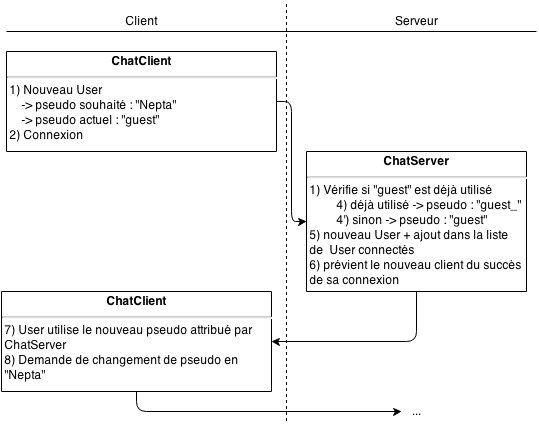
\includegraphics[width=0.7\textwidth]{img/chat_connection.png}
	\caption{Connexion \& identification d'un nouvel utilisateur}
\end{figure}

Cette identification pose plusieurs problèmes :
\begin{itemize}
	\item double affichage d'un message de changement de pseudonyme (guest, et pseudo souhaité);
	\item peu clair au niveau du code;
	\item l'identification est effectuée au niveau du chat, il serait cependant plus judicieux qu'un nouveau module ou que SwitchServer se charge de cette étape.
\end{itemize}

Une piste d'amélioration aurait été d'utiliser un module à part pour l'identification comme suggéré plus haut, ainsi que l'utilisation d'entiers pour identifier les joueurs plutôt que d'utiliser leurs pseudonymes.\\

Une fois connecté, l'utilisateur peut envoyer des messages et des commandes sur le chat via la zone de texte prévue à cet effet. Les commandes sont des classes héritant de AbstractCmd et doivent redéfinir les méthodes \emph{execute} et \emph{getHelp} qui correspondent respectivement à ce que va faire la commande et le message d'aide associé à celle-ci. Comme précisé précédemment, certaines commandes peuvent être lancées depuis le chat à l'aide d'une chaîne de caractères suivant le modèle suivant : \emph{/nom\_commande paramètres} \footnote{Ces commandes sont décrites dans la sous-section dédiée au chat dans la section manuel d'utilisation de ce rapport}. D'autres commandes sont exécutées en réponse à une autre commande, c'est par exemple le cas de la commande CmdNicknameAck qui est exécutée par un client en réponse à un paquet envoyé par le serveur lors d'un changement de pseudonyme (CmdNickname).\\

Toutes les commandes sont instanciées dans la classe Commands, qui elle même est instanciée par ChatClient et ChatServer, ainsi ces deux modules peuvent accéder aux commandes en utilisant la hashmap associant un code à une commande. Par exemple, le code \emph{ChatCodes::USERCMD\_HELP} est associé à la commande d'aide CmdHelp.\\
\newpage

\subsection {Base de données}

\begin{figure}[h!]
    \centering
    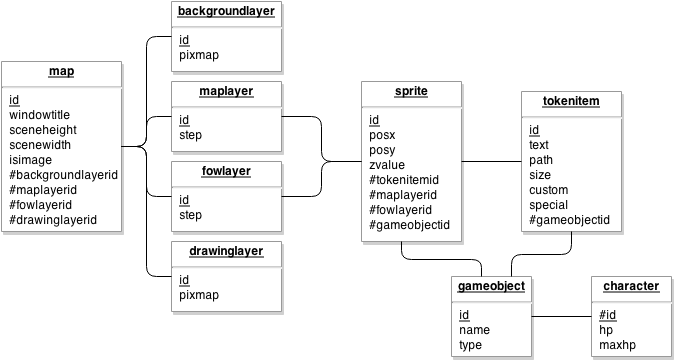
\includegraphics[width=\textwidth]{img/bdd_MLD.png}
    \caption{Modèle Logique des Données}
    \label{fig:bddmld}
\end{figure}

Une base de données PostgreSQL doit être installée avec l'application pour que celle-ci fonctionne correctement. Un script présent dans \textbf{resource/Queries/init.sh} permet d'exécuter les requêtes présentes dans les fichiers initTables.sql et initRows.sql qui, respectivement, permettent de créer les tables et de peupler la base de données. Les tables créées sont modélisées plus haut sur la figure \ref{fig:bddmld}.\\

\begin{figure}[h!]
    \centering
    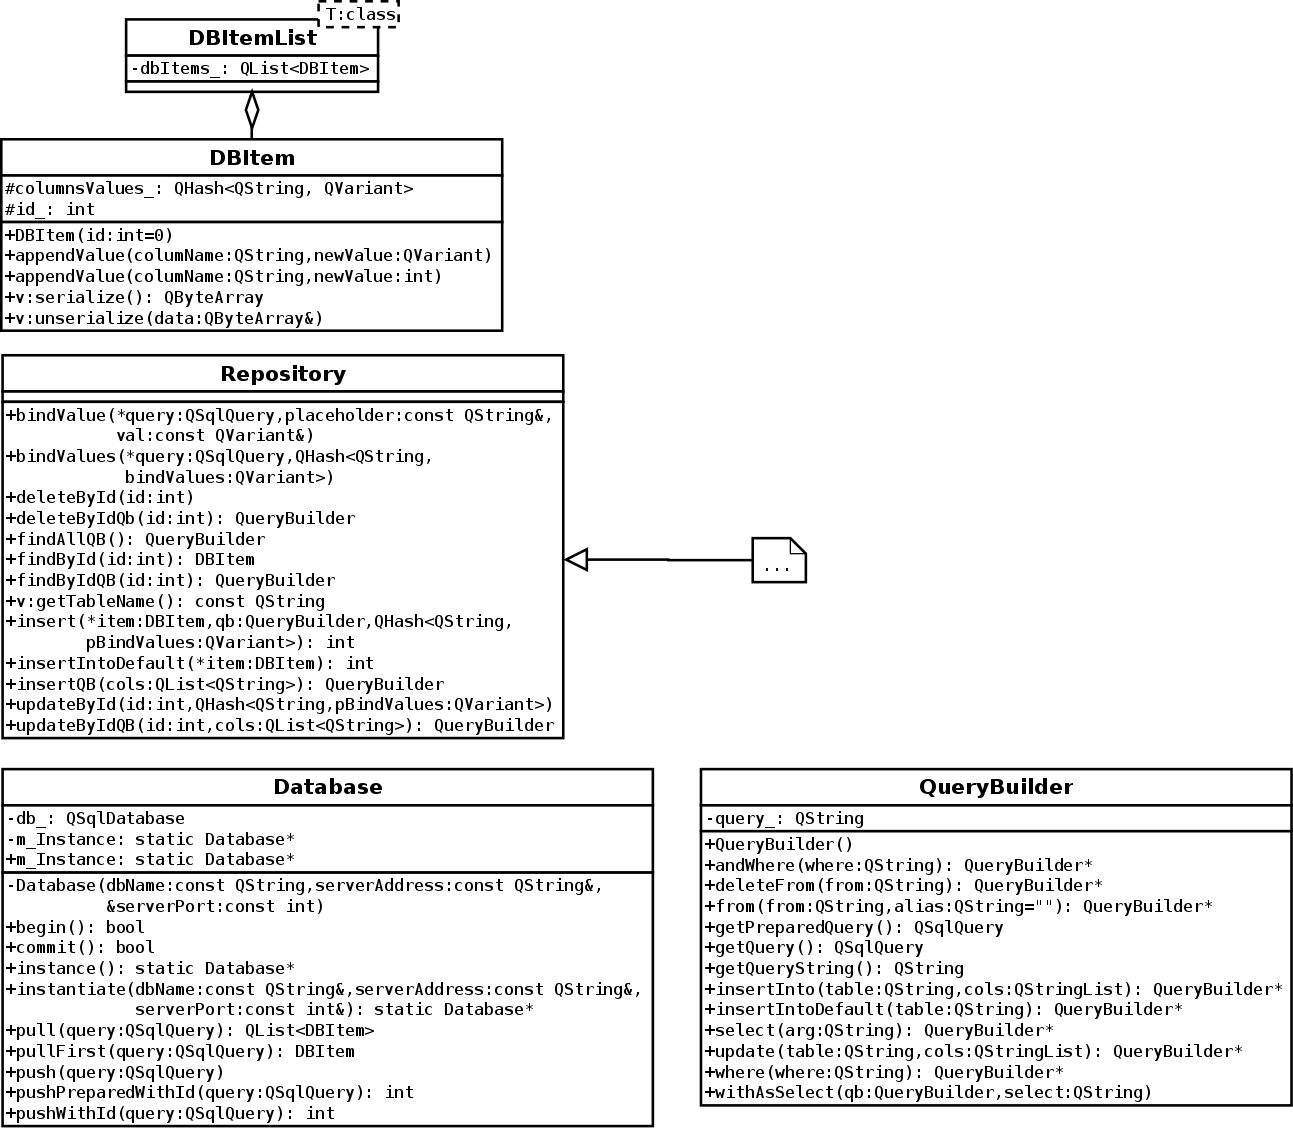
\includegraphics[width=\textwidth]{img/bdd_uml.png}
    \caption{Diagramme UML de la partie BDD (les classes héritant de Repository ne sont pas représentées pour éviter de surcharger le schéma)}
    \label{fig:bdduml}
\end{figure}

La base de données est représentée dans l'application par la classe Database qui a été conçue selon le patron de conception Singleton : Database ne peut être instanciée qu'une seule fois. De plus cette instance est accessible à l'ensemble de l'application ce qui évite de devoir passer cette dépendance à un nombre important de classes. Cette classe permet d'effectuer plusieurs opérations sur la bdd PostgreSQL telles que la récupération d'une seule ligne (\emph{pullFirst}), de plusieurs lignes (\emph{pull}), l'exécution d'une requête ne renvoyant pas de résultat (\emph{push}), et l'exécution d'une requête effectuant une opération d'insertion et renvoyant l'id de la ligne insérée (\emph{pushWithId}).\\

Une classe QueryBuilder a été créée afin de faciliter la création de requêtes. Elle permet de concaténer plusieurs chaînes de caractères afin de former une requête complète. Ainsi, des parties de requêtes peuvent facilement être réutilisées et ainsi éviter de la duplication de code.

\begin{lstlisting}[caption=Exemple d'utilisation de QueryBuilder]
QueryBuilder Repository::findByIdQB(int id) {
    QueryBuilder qb;

    qb.select("*")
    ->from(getTableName())
    ->where("id = " + QString::number(id));

    return qb;
}
\end{lstlisting}

\begin{lstlisting}[language=SQL,caption=Equivalent en SQL de la requête créée avec le QueryBuilder]
SELECT * FROM nomDeLaTable 
WHERE id = idDeLaLigne;
\end{lstlisting}

Ces requêtes sont créées dans des classes héritant de Repository. Un Repository et les classes qui en héritent sont des conteneurs de requêtes. La classe de base Repository possède quelques méthodes génériques qui permettent par exemple de récupérer un élément de la base de données par son id (\emph{findById}), ou encore d'insérer une ligne dans la BDD (\emph{insert}). Les classes héritant de Repository peuvent ensuite redéfinir et/ou réutiliser ces méthodes pour les adapter à leurs besoins. Chaque classe pouvant manipuler des objets associés dans la BDD possède un Repository, par exemple la classe Sprite est associée à la table sprite de la BDD et peut manipuler cette table à l'aide des requêtes de SpriteRepository. Enfin, tous les repositories sont accessibles de manière statique depuis la classe RepositoryManager, ainsi toute l'application a accès à ceux-ci.\\

Les classes possédant une table équivalente en BDD (par exemple la classe TokenItem est liée à la table tokenitem) héritent de DBItem. Un DBItem possède une hashmap associant un nom de colonne à sa valeur. Cette hashmap est remplie et sérialisée avant une insertion en base de données, et déserialisée lors de la récupération de lignes de la BDD.
\newpage

\subsection{Éléments de jeu}

% TODO insérer schéma UML
% 	- GameObject hérite de DBItem
%	- Sprite & Character utilisent GameObject
%	- GameObjectRepository
%	- GameObjectSubRepository <- CharacterRepository

Un élément de jeu est représenté par la classe GameObject. Cette classe hérite de DBItem afin de pouvoir être sérialisée pour être insérée dans la base de données, et désérialisée pour pouvoir reconstruire l'objet après récupération d'informations dans la base de données. Un GameObject possède un nom ainsi qu'un type afin de savoir quel type d'objet doit être inséré/reconstruit en base de données. De plus, cette classe est liée à la table \emph{gameobject} de la bdd, et les requêtes liées à celles-ci sont stockées dans la classe GameObjectRepository.\\

Un Character est un GameObject et représente un personnage dans le jeu. Un Character ne possède que des points de vie pour le moment mais pourrait posséder d'autres éléments tels que des caractéristiques (force, agilité, ...). Cette classe est liée à la table \emph{character} de la bdd, et les requêtes liées sont stockées dans la classe CharacterRepository.\\

Les éléments de jeu sont utilisés dans les TokenItems et les Sprites. A la création d'un Sprite (lors d'un ajout sur la carte) le GameObject possédé par le TokenItem associé au Sprite est copié dans ce dernier.\\

% TODO fait doublon avec bdd_MLD plus haut
\begin{figure}[h!]
        \centering
        \begin{subfigure}[h!]{0.7\textwidth}
                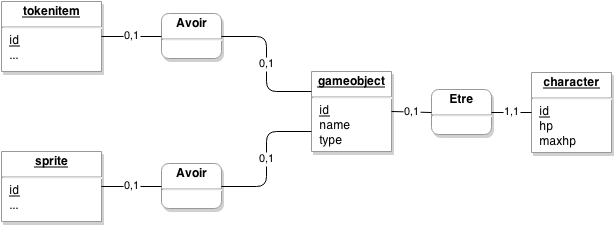
\includegraphics[width=\textwidth]{img/gameobject_MCD.png}
                \caption{Modèle Conceptuel des Données}
        \end{subfigure}

        \begin{subfigure}[h!]{0.5\textwidth}
                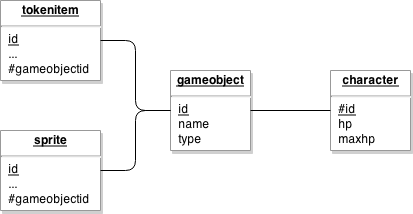
\includegraphics[width=\textwidth]{img/gameobject_MLD.png}
                \caption{Modèle Logique des Données}
        \end{subfigure}
        \caption{MCD et MLD de la base données concernant les GameObjects}
        \label{fig:GameObjectsBDD}
\end{figure}

\newpage

Les Schémas ci-dessus représentent la modélisation de la base de données (MCD et MLD) concernant les GameObjects. Un élément notable est que la table character a pour clé primaire id qui fait référence à une id de la table gameobject. Ainsi, un character et son gameobject lié peuvent être facilement récupérables de la base de données à partir d'une même id.\\

Pour le moment, les seuls éléments de jeu disponibles sont les personnages. Nous pourrions cependant penser à d'autres éléments, par exemple du terrain, ou encore des objets qu'un personnage peut équiper et des consommables.\\
\newpage

\subsection{Les notifications}

Durant l'utilisation de l'application, des notifications sont utilisées pour faire passer des messages de jeu aux joueurs. A chacun de ces événements, une notification s'ajoute sur l'écran puis disparaît après une certaine durée. L'application gère aussi les multiples notifications avec un empileur de notifications. La notification la plus récente s'affichera en dessous de l'ancienne plus récente. \\

L'empileur de notification est une liste de notifications qui commence vide et une notification s'y ajoute lorsque que cela est voulu. A partir du moment où la première notfication est ajoutée, un timer est activé afin d'effacer la notification après la durée prédéterminée. Le timer est stoppé lorsque l'empileur est vide pour que lorsqu'une première notification s'ajoute, elle ne disparaisse pas parce qu'elle a été ajoutée juste avant la fin de la durée. A chaque événement produit par le timer, les notifications sont remontées vers le haut afin de garder l'ordre d'apparition des notifications. Ainsi, nous évitons des superpositions de notifications ou des mélanges de position entre les anciennes ou récentes notifications.

\begin{figure}[h!]
	\centering
	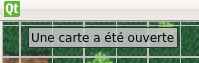
\includegraphics[width=0.3\textwidth]{img/notification.png}
	\caption{Notification lors de l'ouverture d'une carte}
	\label{fig:notification}
\end{figure}
\newpage

\subsection{Cartes et images}

\begin{figure}[h!]
	\centering
	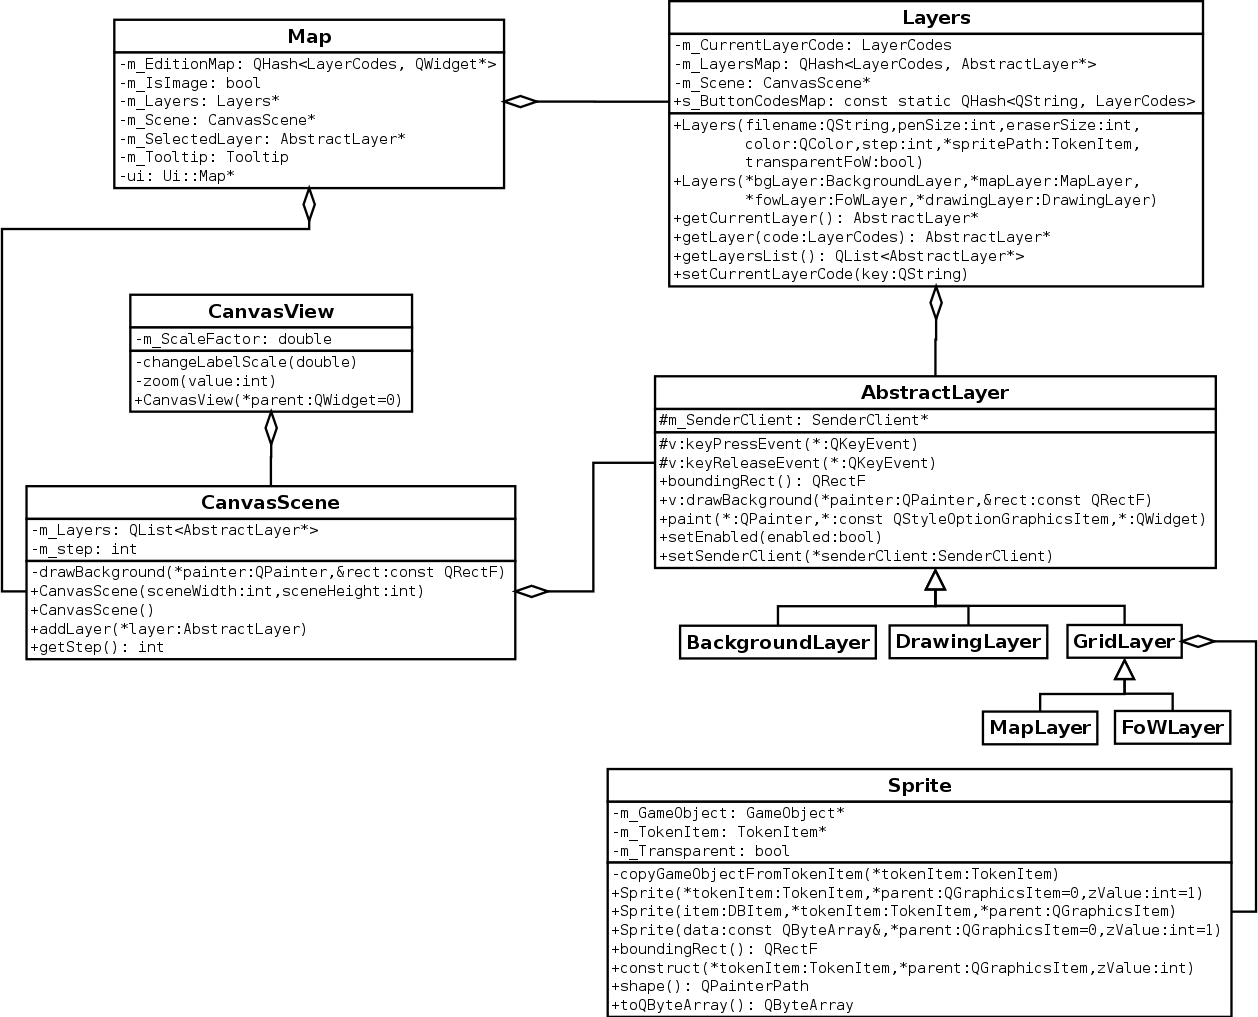
\includegraphics[width=\textwidth]{img/map_uml.png}
	\caption{Diagramme UML de la carte (certaines méthodes sont cachées pour plus de lisibilité)}
\end{figure}

Une image est une carte dont les layers de brouillard de guerre et de personnages sont dissimulés, ainsi que les menus qui leurs sont associés.\\
Une Map hérite de QWidget, afin d'être mise dans une fenêtre, ainsi que de DBItem et SenderHandler pour la mise en réseau. Elle comporte une QGraphicsView, qui sert à afficher une QGraphicsScene comportant différents Layers. Les Layers sont des couches empilées et indépendantes les unes des autres.\\
La classe Map se contente de créer la carte et d'interagir avec la base de données. La création des différents Layers est laissée à la classe Layers, qui possède une QHash associant les layers aux éléments de l'interface utilisateur.\\

Afin d'être placés sur une QGraphicsscene, les Layers sont des QGraphicsObject. Ils sont organisés comme suit:
\begin{description}
	\item[AbstractLayer]: classe abstraite utilisée pour empiler des éléments dans une scène. Réimplémente boundingRect() et paint() de QGraphicsObject. Afin de pouvoir empêcher un Layer d'intercepter les évènements, il possède une méthode setEnable(bool) qui permet de déterminer si le boundingRect doit renvoyer la totalité de la scène ou un point nul.
	\item[GridLayer]: classe abstraite utilisée pour positionner des sprites sur la scène, qui seront alignés sur une grille. Gère aussi l'ajout desdits sprites à la BDD. Enfin, elle interprète les évènements de la souris, pour ajouter ou retirer des sprites.
	\item[BackgroundLayer]: hérite directement d'AbstractLayer, et se contente de peindre un arrière plan sur la scène.
	\item[MapLayer]: hérite de GridLayer, et sert à positionner les jetons sur la carte. En plus de réimplémenter la gestion des évènements à la souris, ce Layer gère des actions de drag and drop. Il  permet aussi d'afficher les informations sur les sprites (points de vie et hauteur de la pile de jetons).
	\item[FoWLayer]: hérite de GridLayer, et sert à positionner les sprites de brouillard de guerre. Ces sprites peuvent être opaques ou transparents selon la valeur d'un booléen dans le constructeur. Ce Layer ne modifie pas l'interprétation des évènements de la souris de GridLayer. Possède deux méthodes pour remplir ou vider la carte de son brouillard de guerre. 
	\item[DrawingLayer]: hérite directement de AbstractLayer. Contient une QPixmap, originellement vide, sur laquelle l'utilisateur pourra dessiner. Afin de gérer les évènements de la souris de manières complètement différentes, ce Layer installe les eventFilter depuis des Tools. Ces Tools sont organisés de manière similaires aux Layers: une classe AbstractTool, différentes classes concrètes de Tools, et une liste Tools qui construit les Tools et permet de les associer à un bouton de l'interface graphique.
\end{description}

\subsection{Les logs}

Le système de log est un module  connecté au réseau, chaque joueur doit donc recevoir les action effectuées par les autre joueurs.
Pour ce faire, ce système est décomposé en 3 parties,  \textit{LogClient}, \textit{LogServer} et \textit{LogGui},
cette dernière partie ne s'occupant que de l'affichage.

Lorsqu'un joueur effectue une action (ajout, déplacement ou suppression d'un sprite), le gestionnaire de cartes informe le gestionnaire de logs à travers le \textit{LogClient}.
Celui ci permet, avec le \textit{LogServer} la communication des différentes interfaces de jeu.
Le \textit{LogServer} reçoit les information des différents \textit{LogClient} et les réexpédie à tous les clients.
Une fois cela fait, les \textit{LogClient} qui reçoivent maintenant des informations de tous les joueurs peuvent, par le biais du \textit{LogGui} afficher les différentes actions dans un widget prévu à cet effet.
A terme nous aurions pû utiliser cet historique à des fins de contrôle plus poussé, en permettant directement l'annulation des actions depuis ce menu ou encore un affichage pour la gestion de permission (essayer pour un joueur de déplacer son jeton si il n'a plus de vie afficherait un message d'erreur dans les logs).

\newpage

\newpage

\section{Conclusion}

Nous avons implémenté l'ensemble des fonctionnalités qui nous avaient été demandées, à savoir:
\begin{description}
	\item[Création de la partie par le MJ]: chargement des cartes, placement des ennemis sur chaque carte, chargement des documents
	\item[Geston de la partie]: placements et déplacements des personnages, découverte de la carte en cours gérée par le MJ, gestion du temps, génération de lancés de dés
	\item[Mise en réseau du projet]
\end{description}
\hfill

De plus, nous avons ajouté quelques fonctionnalités, telles que:
\begin{description}
	\item[Chat]: mise en place d'un système de messagerie adapté aux besoins du jeu de rôle
	\item[Logs]: afin d'assurer un meilleur suivi de la partie par le MJ
	\item[Éléments de jeu]: afin de rendre plus pratique le suivi des personnages par le MJ
	\item[Possibilité de dessiner]: pour que les utilisateurs retrouvent toutes les possibilités offertes par les cartes papier
\end{description}
\hfill

Cependant, nous avons aussi pensé à ajouter quelques fonctionnalités, et ne sommes pas satisfaits par la généricité de certains éléments de code:
\begin{description}
	\item[Code]: nous aurions préféré utiliser le pattern Builder pour créer les différentes Map, plutôt que d'avoir de multiples constructeurs. De plus, nous aurions souhaité avoir des Actions génériques communes à tous les modules réseau, comme précisé dans la partie Réseau. Enfin, nous aurions souhaité que l'identification ne se fasse pas par le Chat.
	\item[Fonctionnalités]: nous avons souhaité implémenter des curseurs différents pour le mode de dessin des cartes, pouvoir revenir en arrière à l'aide des logs et d'une refonte pour avoir des Actions, et avoir un système de modération pour limiter les actions des joueurs selon l'envie du MJ. De plus, nous aurions pu ajouter des commandes supplémentaires dans le chat, un historique des commandes du chat et faire un paquet pour l'application.
\end{description}
\newpage

\end{document}